\documentclass[12pt,a4paper]{report}

\usepackage{indentfirst}
\usepackage{graphicx}
\usepackage{amsmath, amssymb}
\usepackage{hyperref}
\usepackage{geometry}
\usepackage{caption}
\usepackage{subcaption}

\geometry{a4paper, margin=1in}

\title{
    \vspace{3cm}
    \textbf{Experiment Report}\\[0.5cm]
    \Large Computer-Aided Geometric Design\\[0.5cm]
    \vspace{2cm}
}
\author{15 Liu Xing \\ PB22000150}
\date{\today}

\begin{document}
    \maketitle
    \tableofcontents
    \newpage

    \chapter{Introduction}
        \section{Background}
            In Computer-Aided Geometric Design (CAGD), it is often necessary to smoothly connect a set of points. The method that passes through all the given points is called interpolation. In the two-dimensional case, common interpolation approaches include polynomial interpolation and radial basis function (RBF) interpolation, each with its own characteristics and applicability.

        \section{Objectives}
            In this experiment, two algorithms will be implemented. The input point set is determined by mouse clicks, and then interpolation curves are obtained and plotted using the two methods. Since there are many quantitative measures to evaluate the quality of interpolation functions, this experiment relies on visual inspection for comparison. In addition, numerical stability will be compared using extreme point data.

    \chapter{Algorithm Description}
        \section{Polynomial Interpolation}
            Polynomial interpolation involves finding a polynomial of degree $n-1$ that passes through $n$ given points. The Lagrange interpolation formula is commonly used for this purpose. 

            Newton interpolation is a method for constructing polynomial interpolants. The key idea is to use **divided differences** to build the interpolation polynomial step by step.

            Given nodes $\left\{\left(x_{i}, y_{i}\right)\right\}_{i=0}^{n-1}$, the Newton interpolation polynomial can be written as
            \begin{equation*}
                p\left(x\right) = f\left[x_{0}\right] + f\left[x_{0}, x_{1}\right]\left(x - x_{0}\right) + \cdots + f\left[x_{0}, \dots, x_{n}\right]\left(x - x_{0}\right)\left(x - x_{1}\right)\cdots\left(x - x_{n-1}\right)
            \end{equation*}
            where $f\left[x_{i},\dots,x_{j}\right]$ denotes the corresponding divided difference, which can be computed recursively as follows:

            \begin{enumerate}
                \item Zero-order divided differences (function values):
                \begin{equation*}
                    f\left[x_{i}\right] = y_{i} = f\left(x_{i}\right), \quad i = 0, 1 , \dots, n-1
                \end{equation*}
                
                \item First-order divided differences:
                \begin{equation*}
                    f\left[x_{i}, x_{i+1}\right] = \frac{f\left[x_{i+1}\right] - f\left[x_{i}\right]}{x_{i+1} - x_{i}}
                \end{equation*}
                
                \item Higher-order divided differences for $k \ge 2$:
                \begin{equation*}
                    f\left[x_{i}, x_{i+1}, \dots, x_{i+k}\right] = \frac{f\left[x_{i+1}, \dots, x_{i+k}\right] - f\left[x_i, \dots, x_{i+k-1}\right]}{x_{i+k} - x_i}
                \end{equation*}
            \end{enumerate}

            The advantages of Newton interpolation are:

            \begin{itemize}
                \item The interpolation polynomial can be constructed recursively, and when a new node is added, only the new divided difference needs to be computed;
                \item Compared with directly solving the Vandermonde system, it provides better numerical stability.
            \end{itemize}

        \section{Radial Basis Function (RBF) Interpolation}\label{sec:rbf}
            Radial Basis Function (RBF) interpolation is a method that uses radially symmetric functions to approximate data.

            Given nodes $\left\{\left(x_{i}, y_{i}\right)\right\}_{i=1}^n$, the general form of the RBF interpolant is

            
            \begin{equation*}
                s\left(x\right) = \sum_{i=0}^{n-1} b_{i} \, \phi\left(\left\lVert x - x_{i}\right\rVert\right) + p\left(x\right)
            \end{equation*}

            where:
            \begin{itemize}
                \item $\phi\left(r\right)$ is a radial basis function that depends only on the distance $r = \left\lVert x-x_i\right\rVert$, such as $\phi\left(r\right) = \frac{1}{r^2 + d}$ or $\phi\left(r\right) = e^{-\left(\varepsilon r\right)^{2}}$;
                \item The coefficients $b_{i}$ are determined by solving a linear system so that the interpolation conditions $s\left(x_{i}\right) = y_{i}$ are satisfied;
                \item $p\left(x\right)$ is a low-degree polynomial (or a constant term) used as a tail to ensure solvability and improve numerical stability.
            \end{itemize}

            RBF interpolation is advantageous in that it does not rely on mesh structures in higher dimensions and can handle scattered data effectively. However, its numerical stability is sensitive to the choice of kernel parameters (e.g., the shape parameter $d$ or $\varepsilon$).

            In this experiment, we chose $\phi\left(r\right) = \frac{1}{r^{2} + d}$ as the basis function, with $d$ set as a fixed hyperparameter adjustable via a slider. We then set the tail as a constant. Since there are $n+1$ unknowns but only $n$ equations, an additional constraint is required. Here, we impose $\sum_{i=0}^{n-1} b_{i} = 0$ as the constraint, which transforms the system into
            \begin{equation*}
                \begin{bmatrix}
                    A & \mathbf{1} \\
                    \mathbf{1}^{\top} & 0
                \end{bmatrix}
                \begin{bmatrix}
                    \mathbf{b} \\
                    c
                \end{bmatrix}
                =
                \begin{bmatrix}
                    \mathbf{y} \\
                    0
                \end{bmatrix}
            \end{equation*}
            with $A = \left(\phi\left(\left\lVert x_{i} - x_{j}\right\rVert\right)\right)_{n\times n}$. For numerical stability, a term $\lambda I$ is added to $A$ during the actual solution process. This form is convenient for solving because the augmented matrix on the left is symmetric, allowing the use of efficient algorithms for symmetric linear systems and ensuring numerical stability.

    \chapter{Program Explanation}
        \section{Programming Platform}
            This experimental code was written on MATLAB R2024b under the Windows 11 platform, but it is compatible with all MATLAB versions later than R2018b.

        \section{Program Structure}
            The program consists of a single file, which is divided into three sections using the ``\%\%'' delimiter.

            The first section handles the UI plotting logic. Most of it is based on the provided code template, but a logarithmic-scale \texttt{slider} has been added, and the polygon drawing and event-listening logic has been updated to use \texttt{drawpolyline} and \texttt{addlistener} to leverage the newer MATLAB graphics engine and ensure longer-term compatibility.

            The second section implements the polynomial interpolation function using the Newton interpolation method to improve numerical stability and computational efficiency.

            The third section implements the RBF interpolation function, providing interfaces for the shape parameter $d$ and the regularization parameter $\lambda$.


        \section{Program Usage}
            \begin{itemize}
                \item Run the program in MATLAB. A window will pop up with a blank canvas.
                \item You can add points by simply clicking on the canvas. Double-click while adding the last point can complete the polygon and display the interpolation functions fitted by the two methods.
                \item Afterwards, you can drag any of the existing points at any time to change their positions.
                \item A slider for controlling the shape parameter $d$ also appears at the bottom of the screen; dragging it allows you to adjust $d$ in real time within the range $1\times10^{-3} \sim 1\times10^{1}$, and the interpolation plot updates immediately.
            \end{itemize} 

    \chapter{Results}
        \section{General Results}
            To compare the applicability of the two interpolation methods, I analyzed three scenarios: interpolation of nearly linear point sets, fitting of convex point sets, and fitting of oscillatory point sets.

            First, we compare the case of points close to a linear function. Both methods produce satisfactory results; however, polynomial interpolation may exhibit oscillations at the boundaries depending on the parity of the number of points, as shown in Figure~\ref{fig:linear}. Additionally, if several points are very close to each other—resulting in larger differences in pairwise slopes—both methods may exhibit oscillations, as illustrated in Figure~\ref{fig:linear_close}.

            Next, we consider convex point sets. Here, "convex" means that each subsequent point lies above the line connecting the previous two points, rather than the point set itself forming a convex hull. In this scenario, the theoretically expected interpolation should approximate a convex function. Tests show that polynomial interpolation performs better than RBF in this case, as seen in Figure~\ref{fig:convex}. However, increasing the RBF shape parameter $d$ can also produce convex RBF interpolation results, as shown in Figure~\ref{fig:convex_big_d}.

            Finally, we examine oscillatory point sets. Polynomial interpolation exhibits a more pronounced Runge phenomenon, whereas RBF interpolation produces a smoother and more natural curve, as shown in Figure~\ref{fig:runge}. However, in this scenario, increasing the RBF shape parameter $d$ can reduce numerical stability, preventing the interpolated function from passing through the given points, as illustrated in Figure~\ref{fig:runge_big_d}.
            
        \begin{figure}[htbp]
            \centering
            % 第一行
            \subfloat[Nearly linear points]{%
                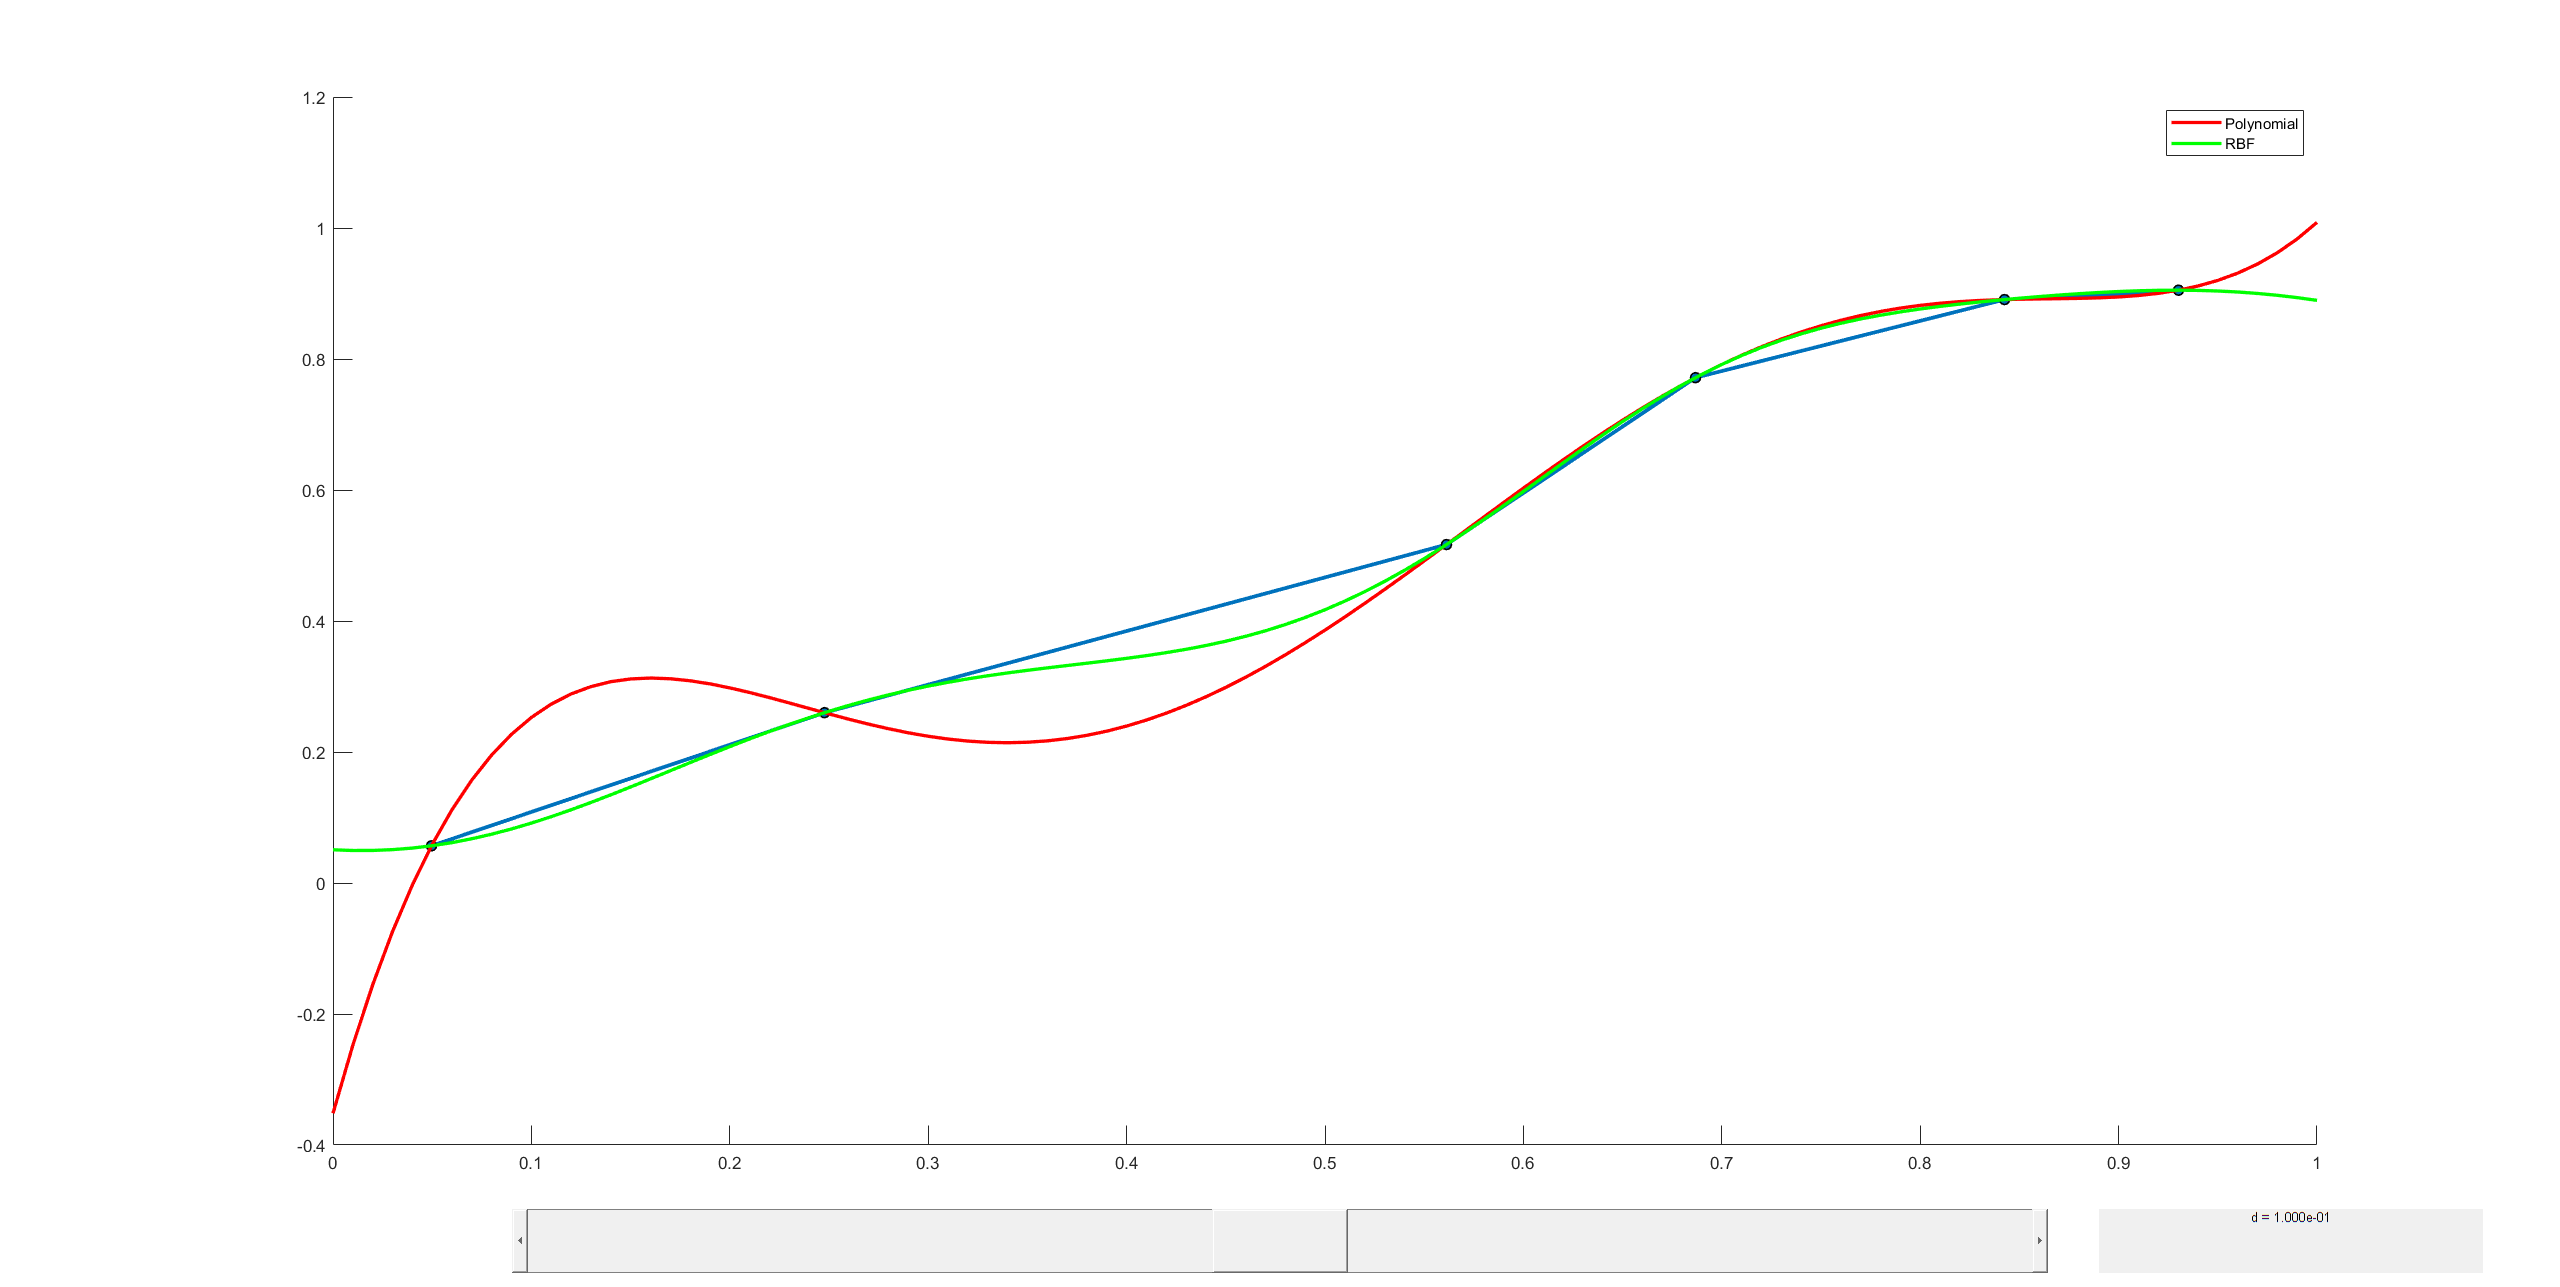
\includegraphics[width=0.45\textwidth]{Figure/00linear.png}%
                \label{fig:linear}%
            }\hfill
            \subfloat[Close points causing oscillation]{%
                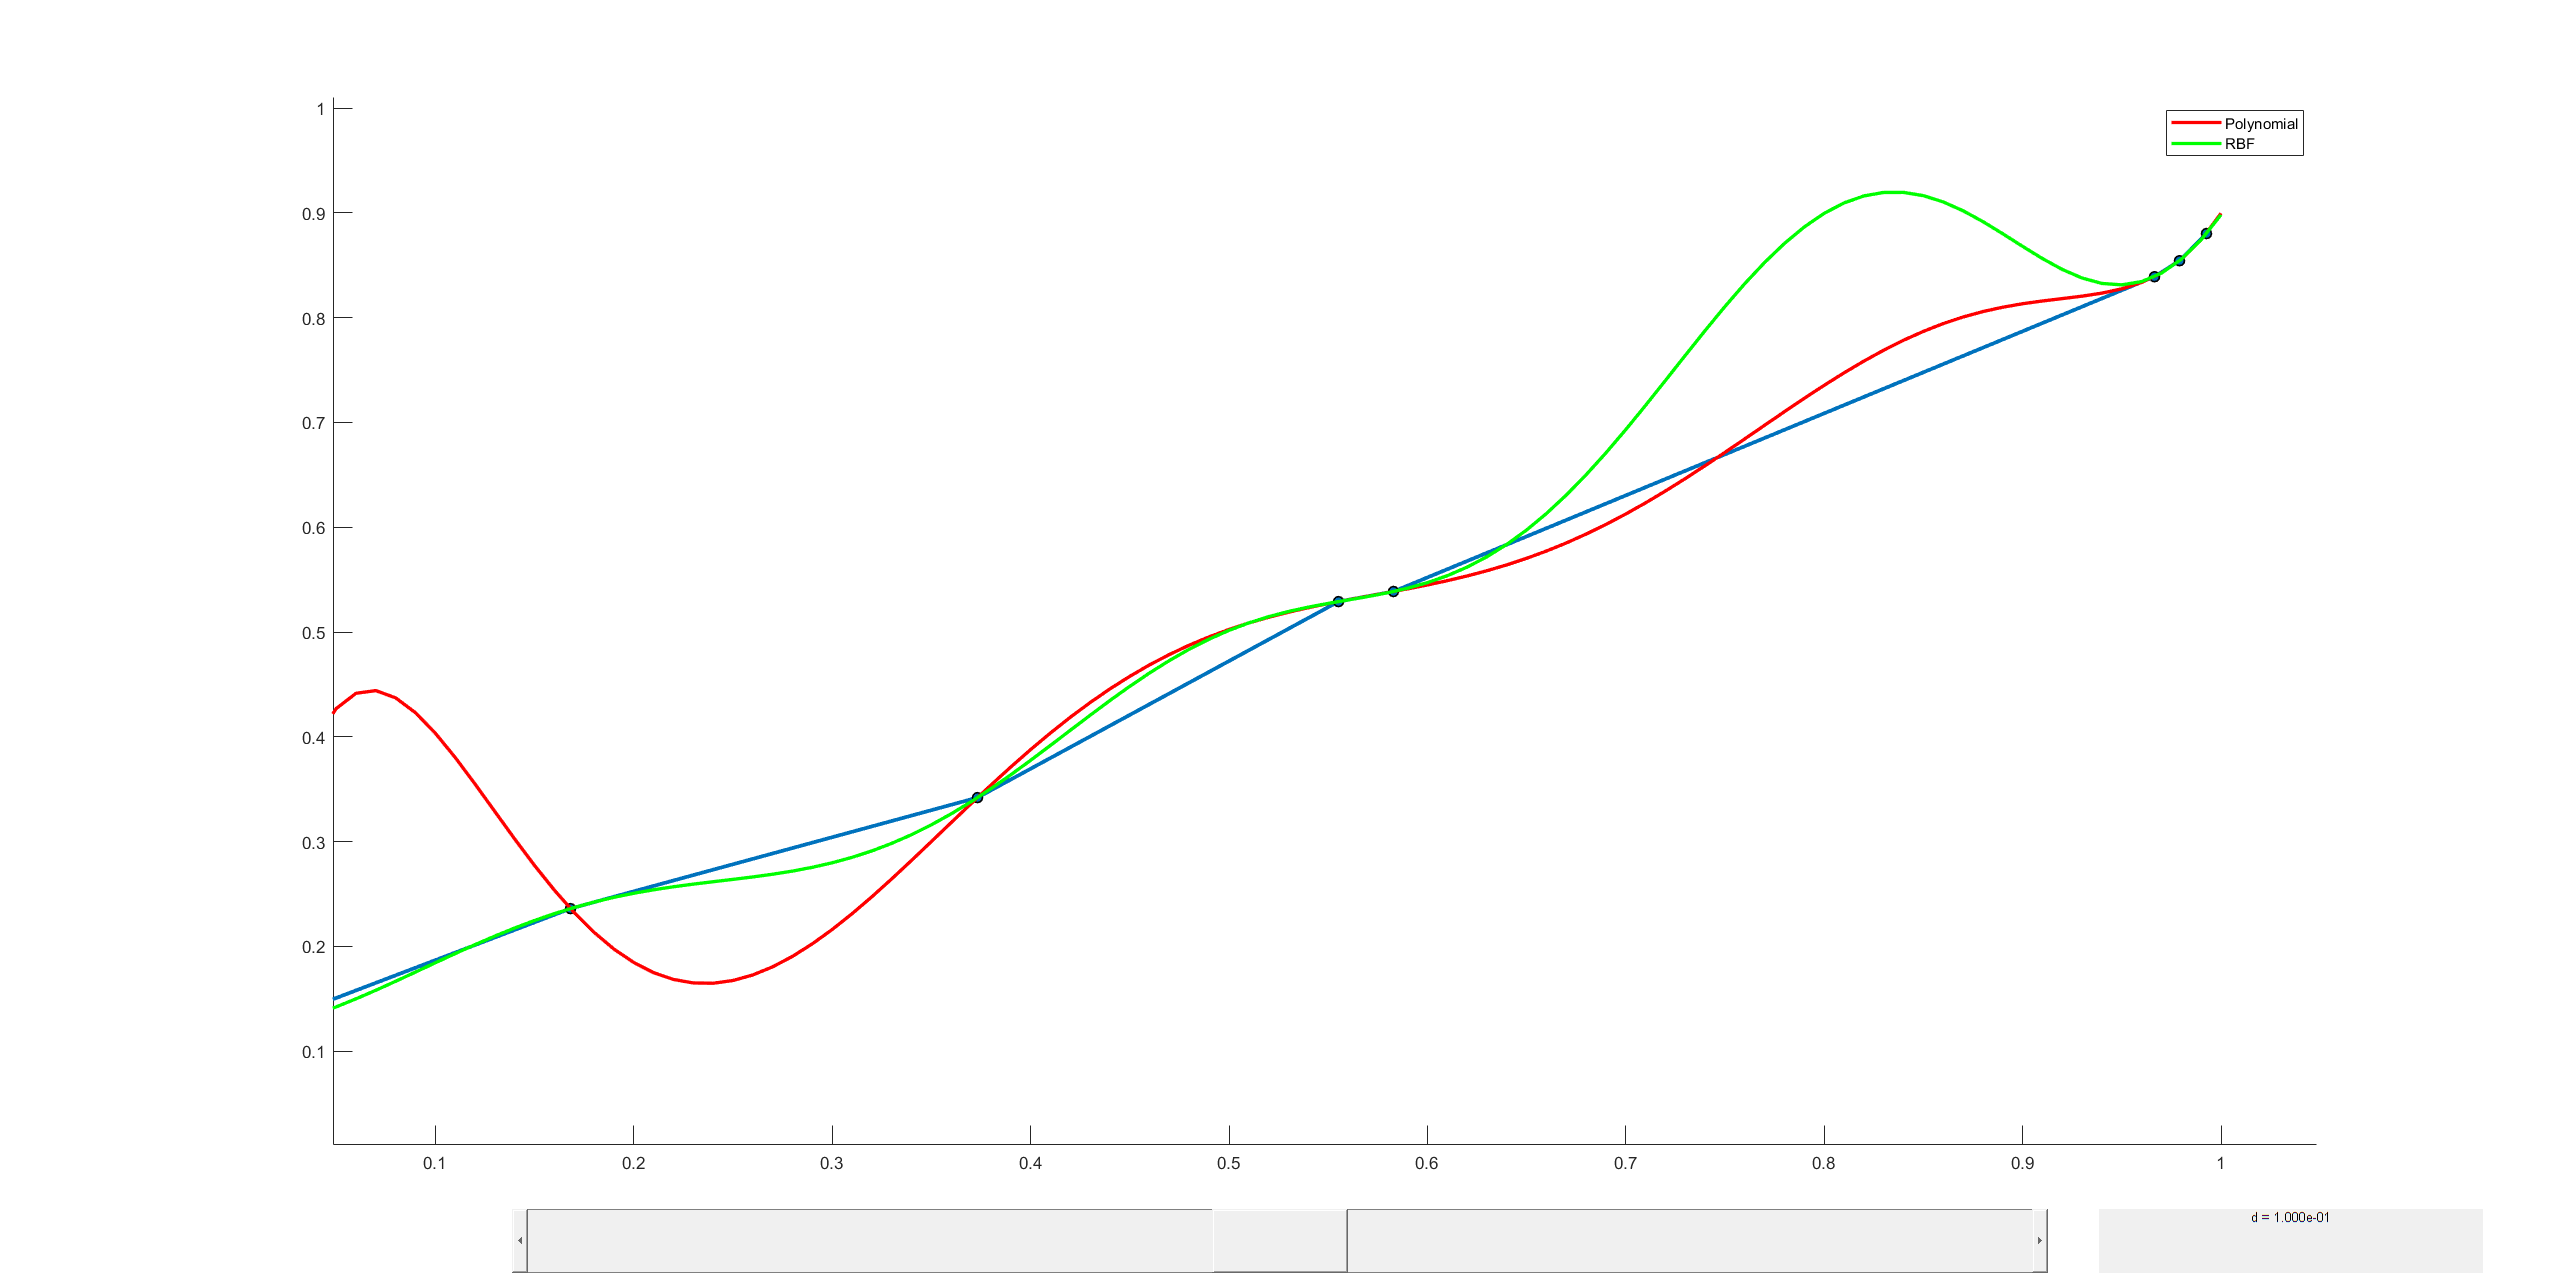
\includegraphics[width=0.45\textwidth]{Figure/01linear_close.png}%
                \label{fig:linear_close}%
            }

            % 第二行
            \subfloat[Convex points]{%
                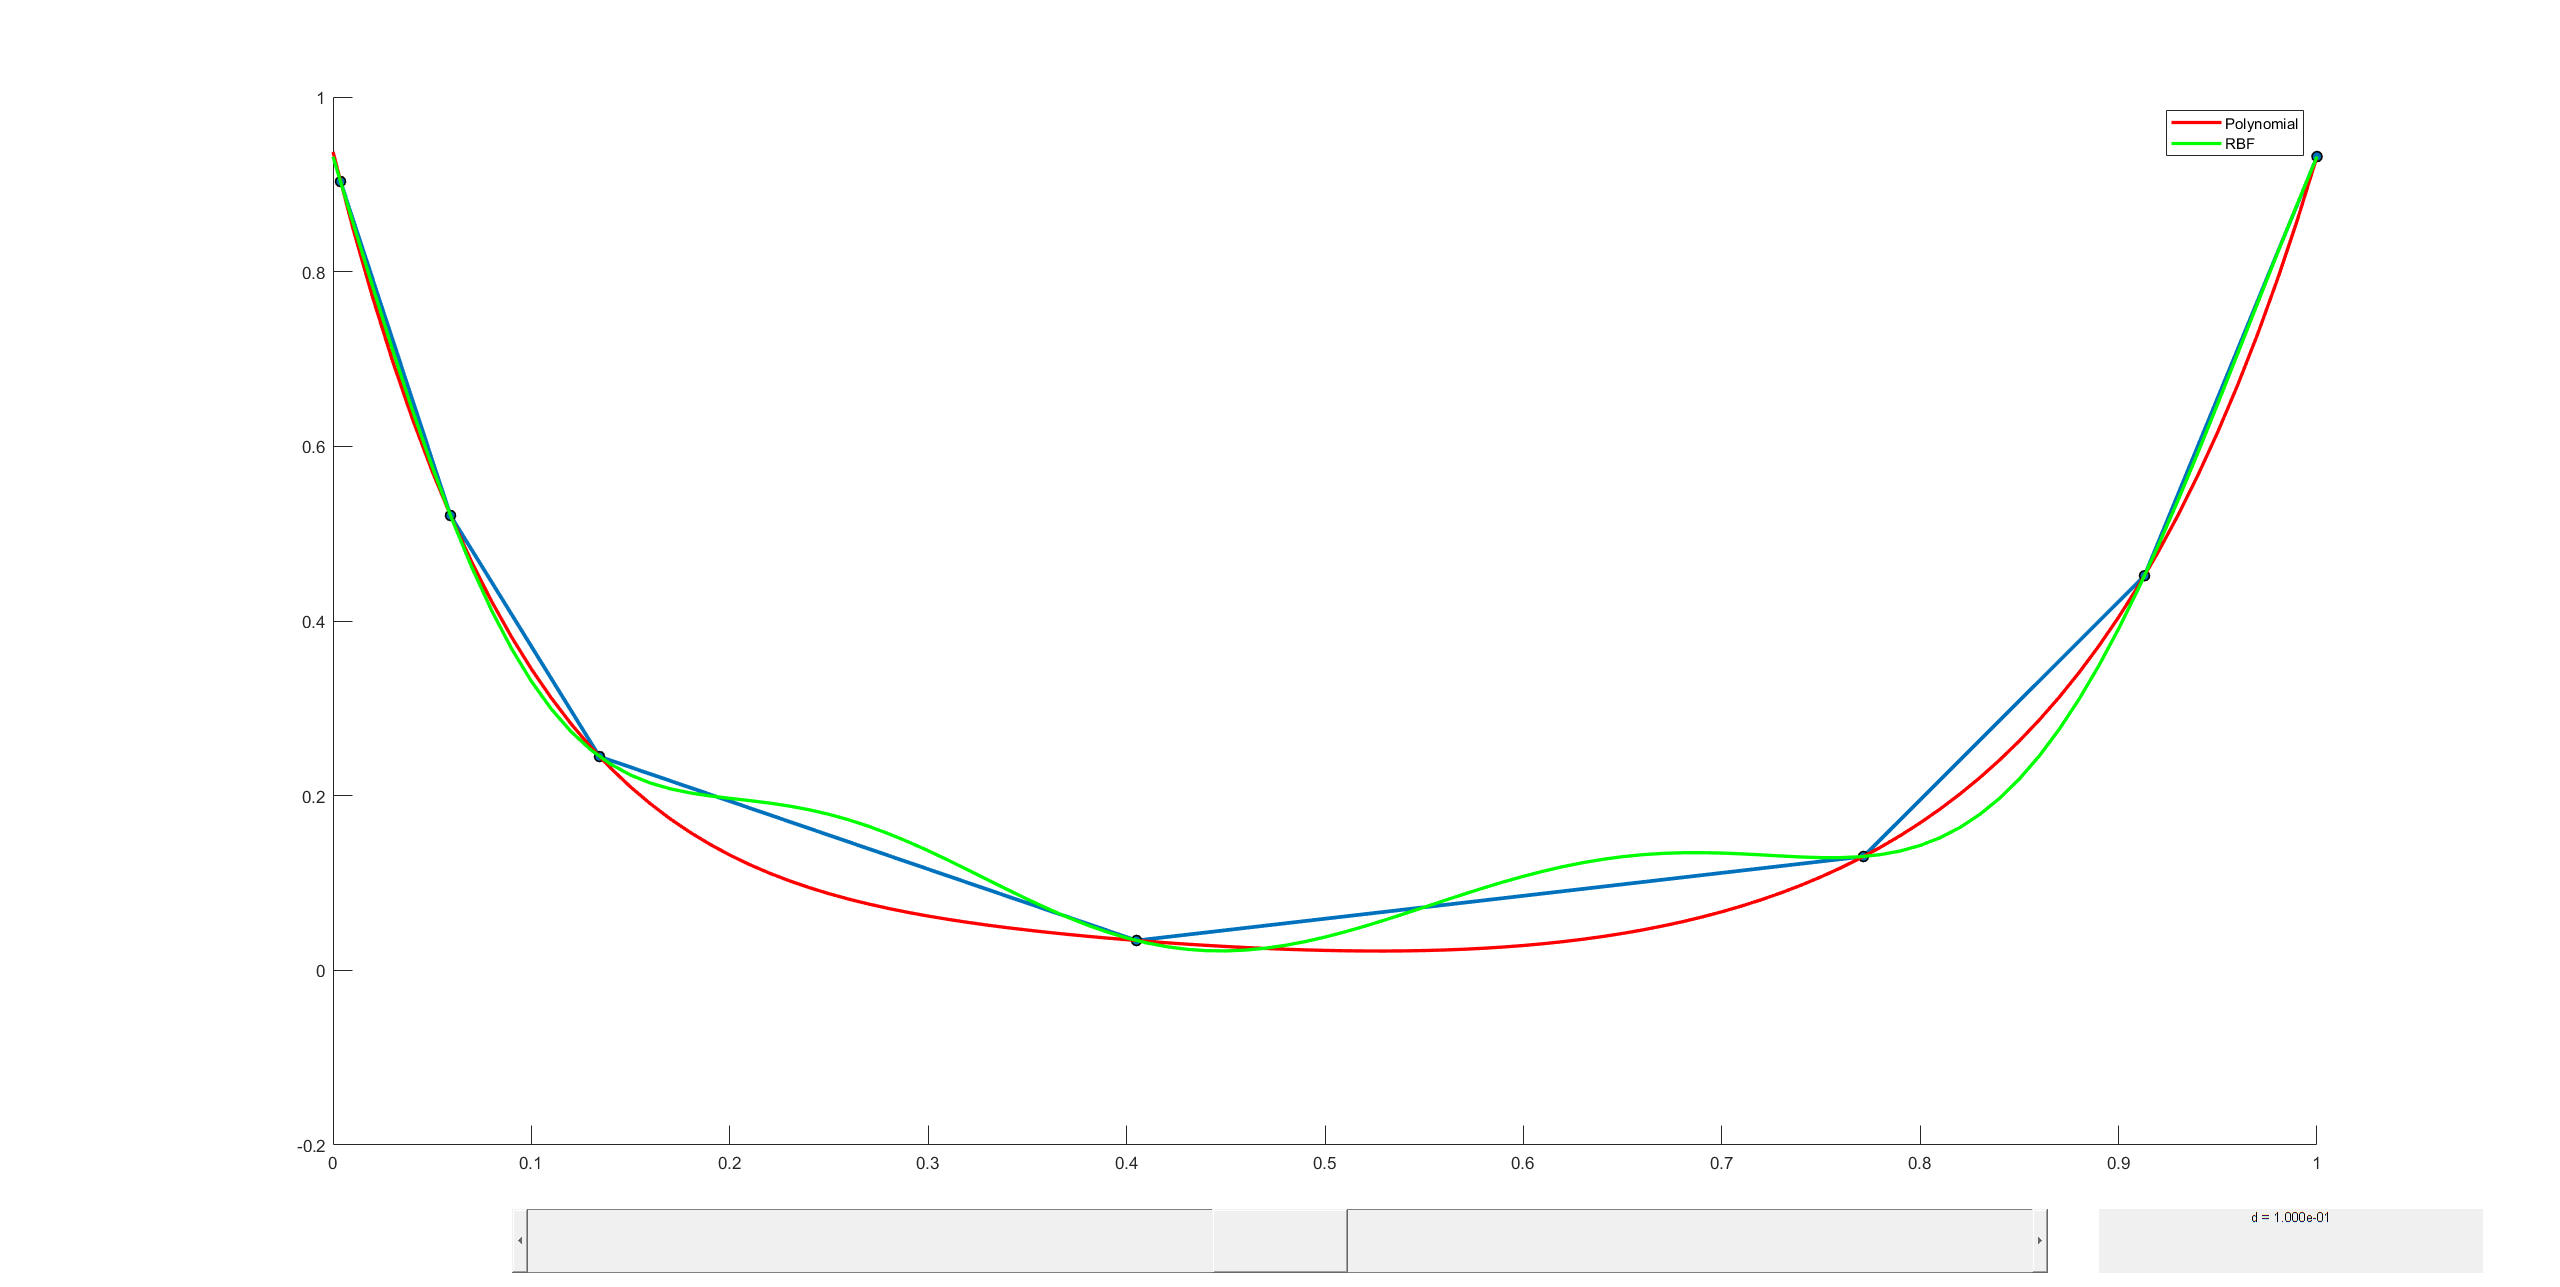
\includegraphics[width=0.45\textwidth]{Figure/10convex.png}%
                \label{fig:convex}%
            }\hfill
            \subfloat[RBF with large d, convex]{%
                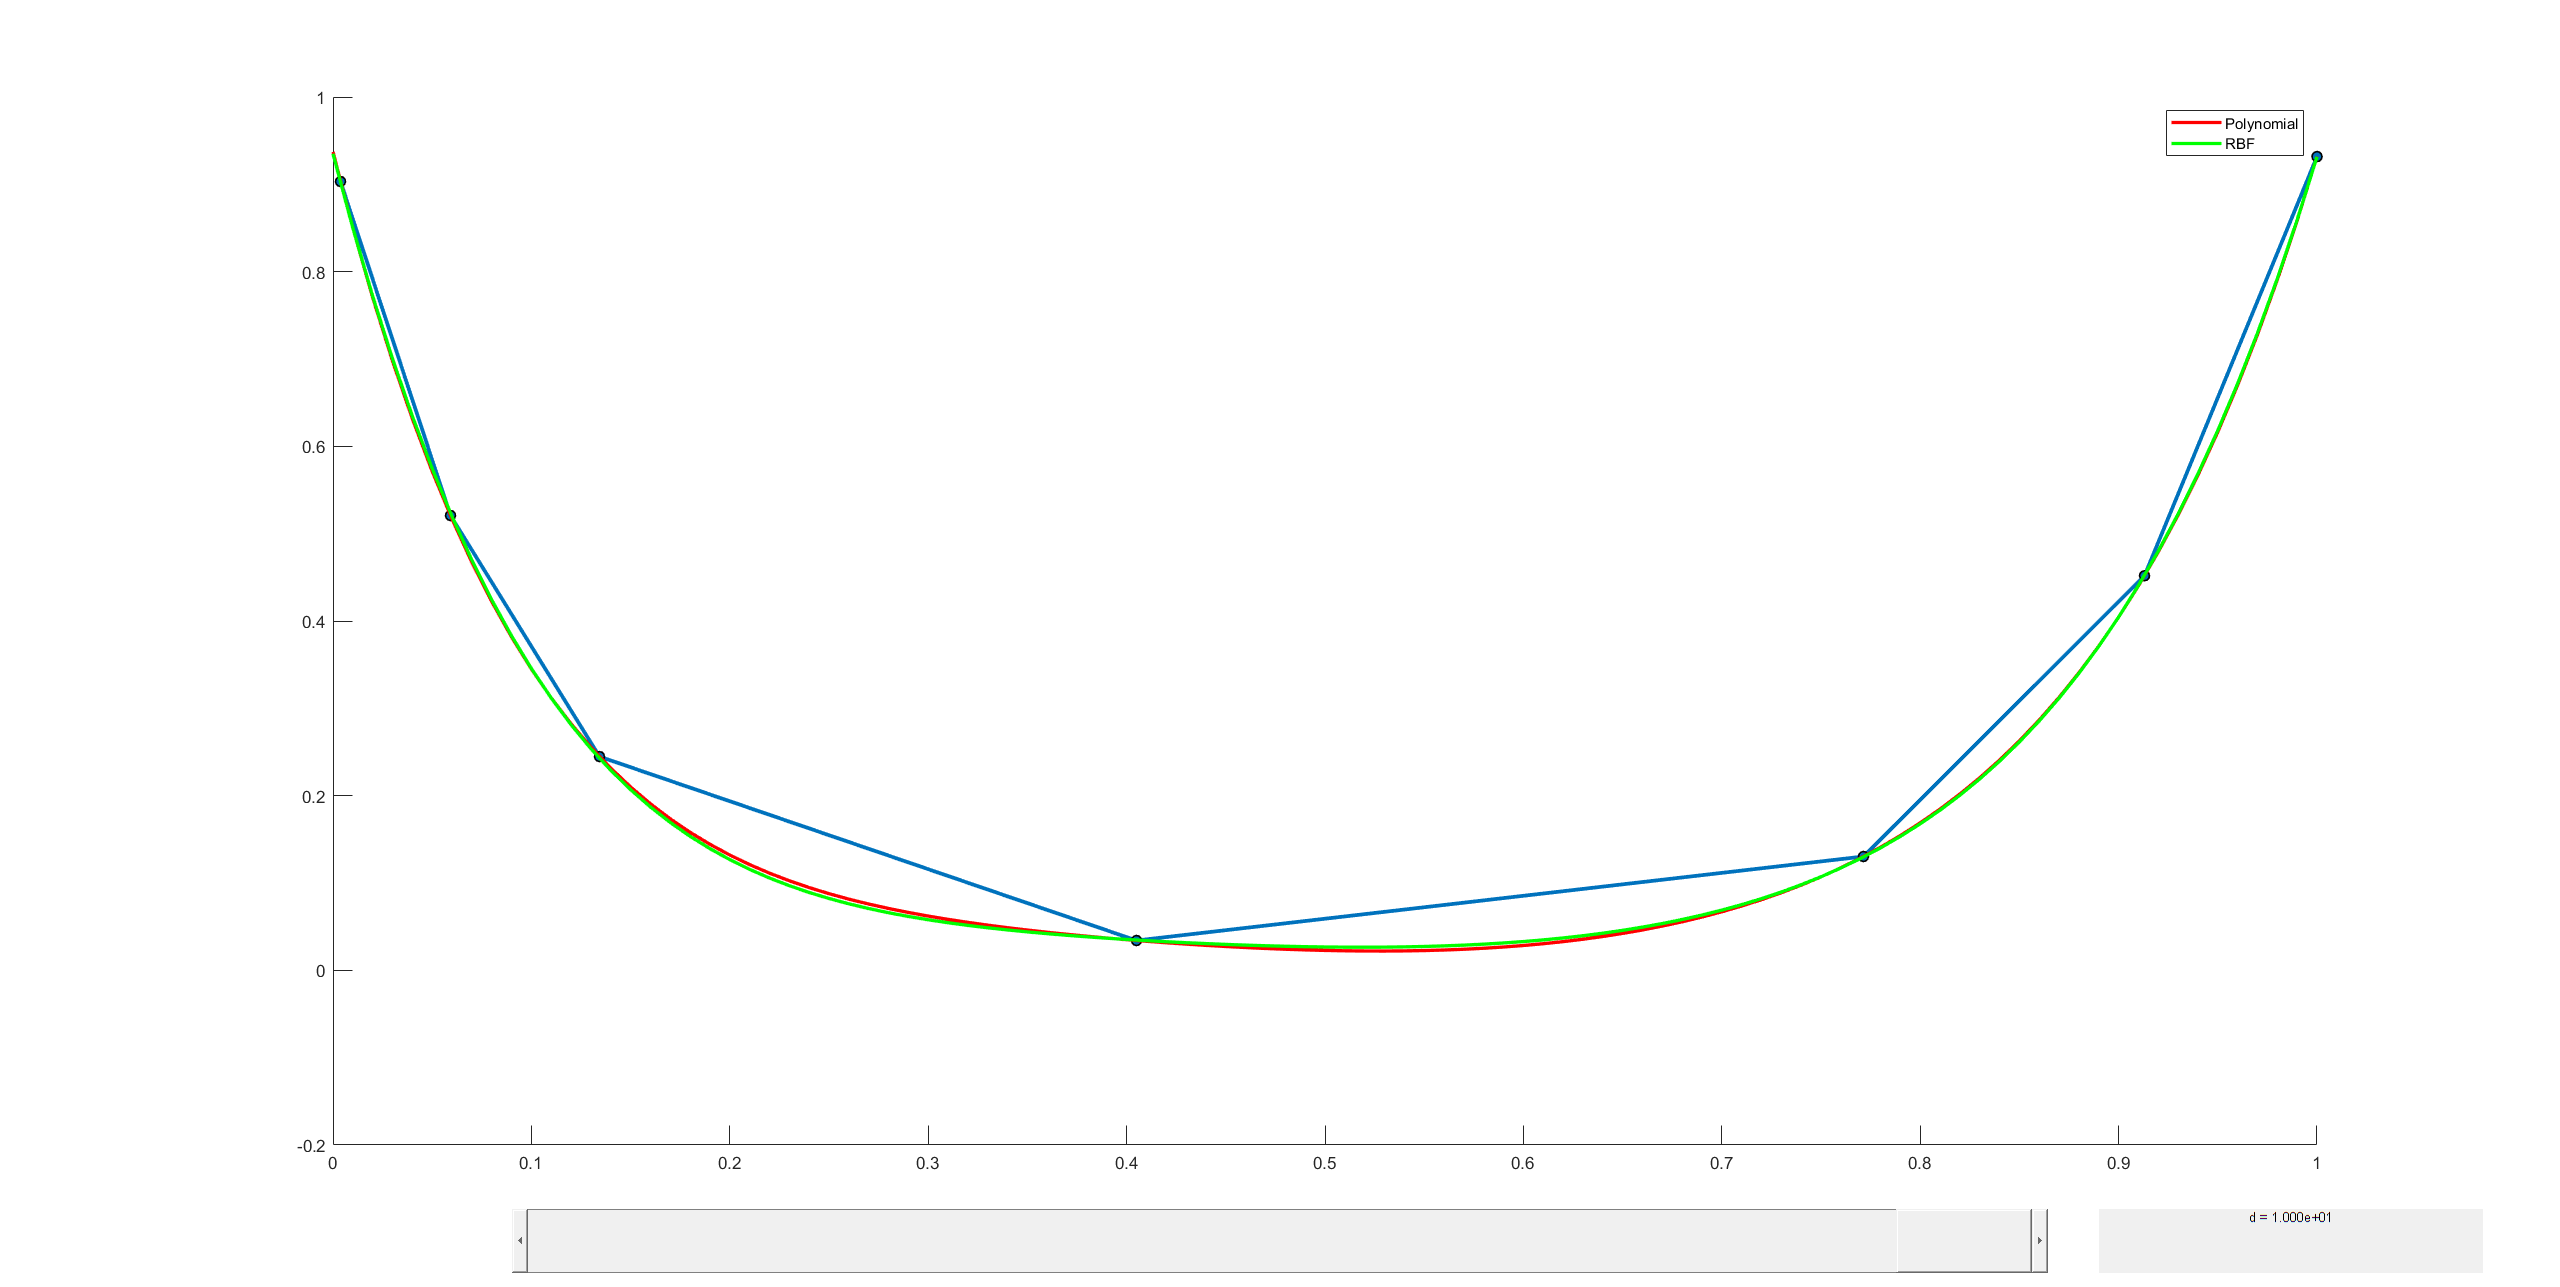
\includegraphics[width=0.45\textwidth]{Figure/11convex_big_d.png}%
                \label{fig:convex_big_d}%
            }

            % 第三行
            \subfloat[Oscillatory points]{%
                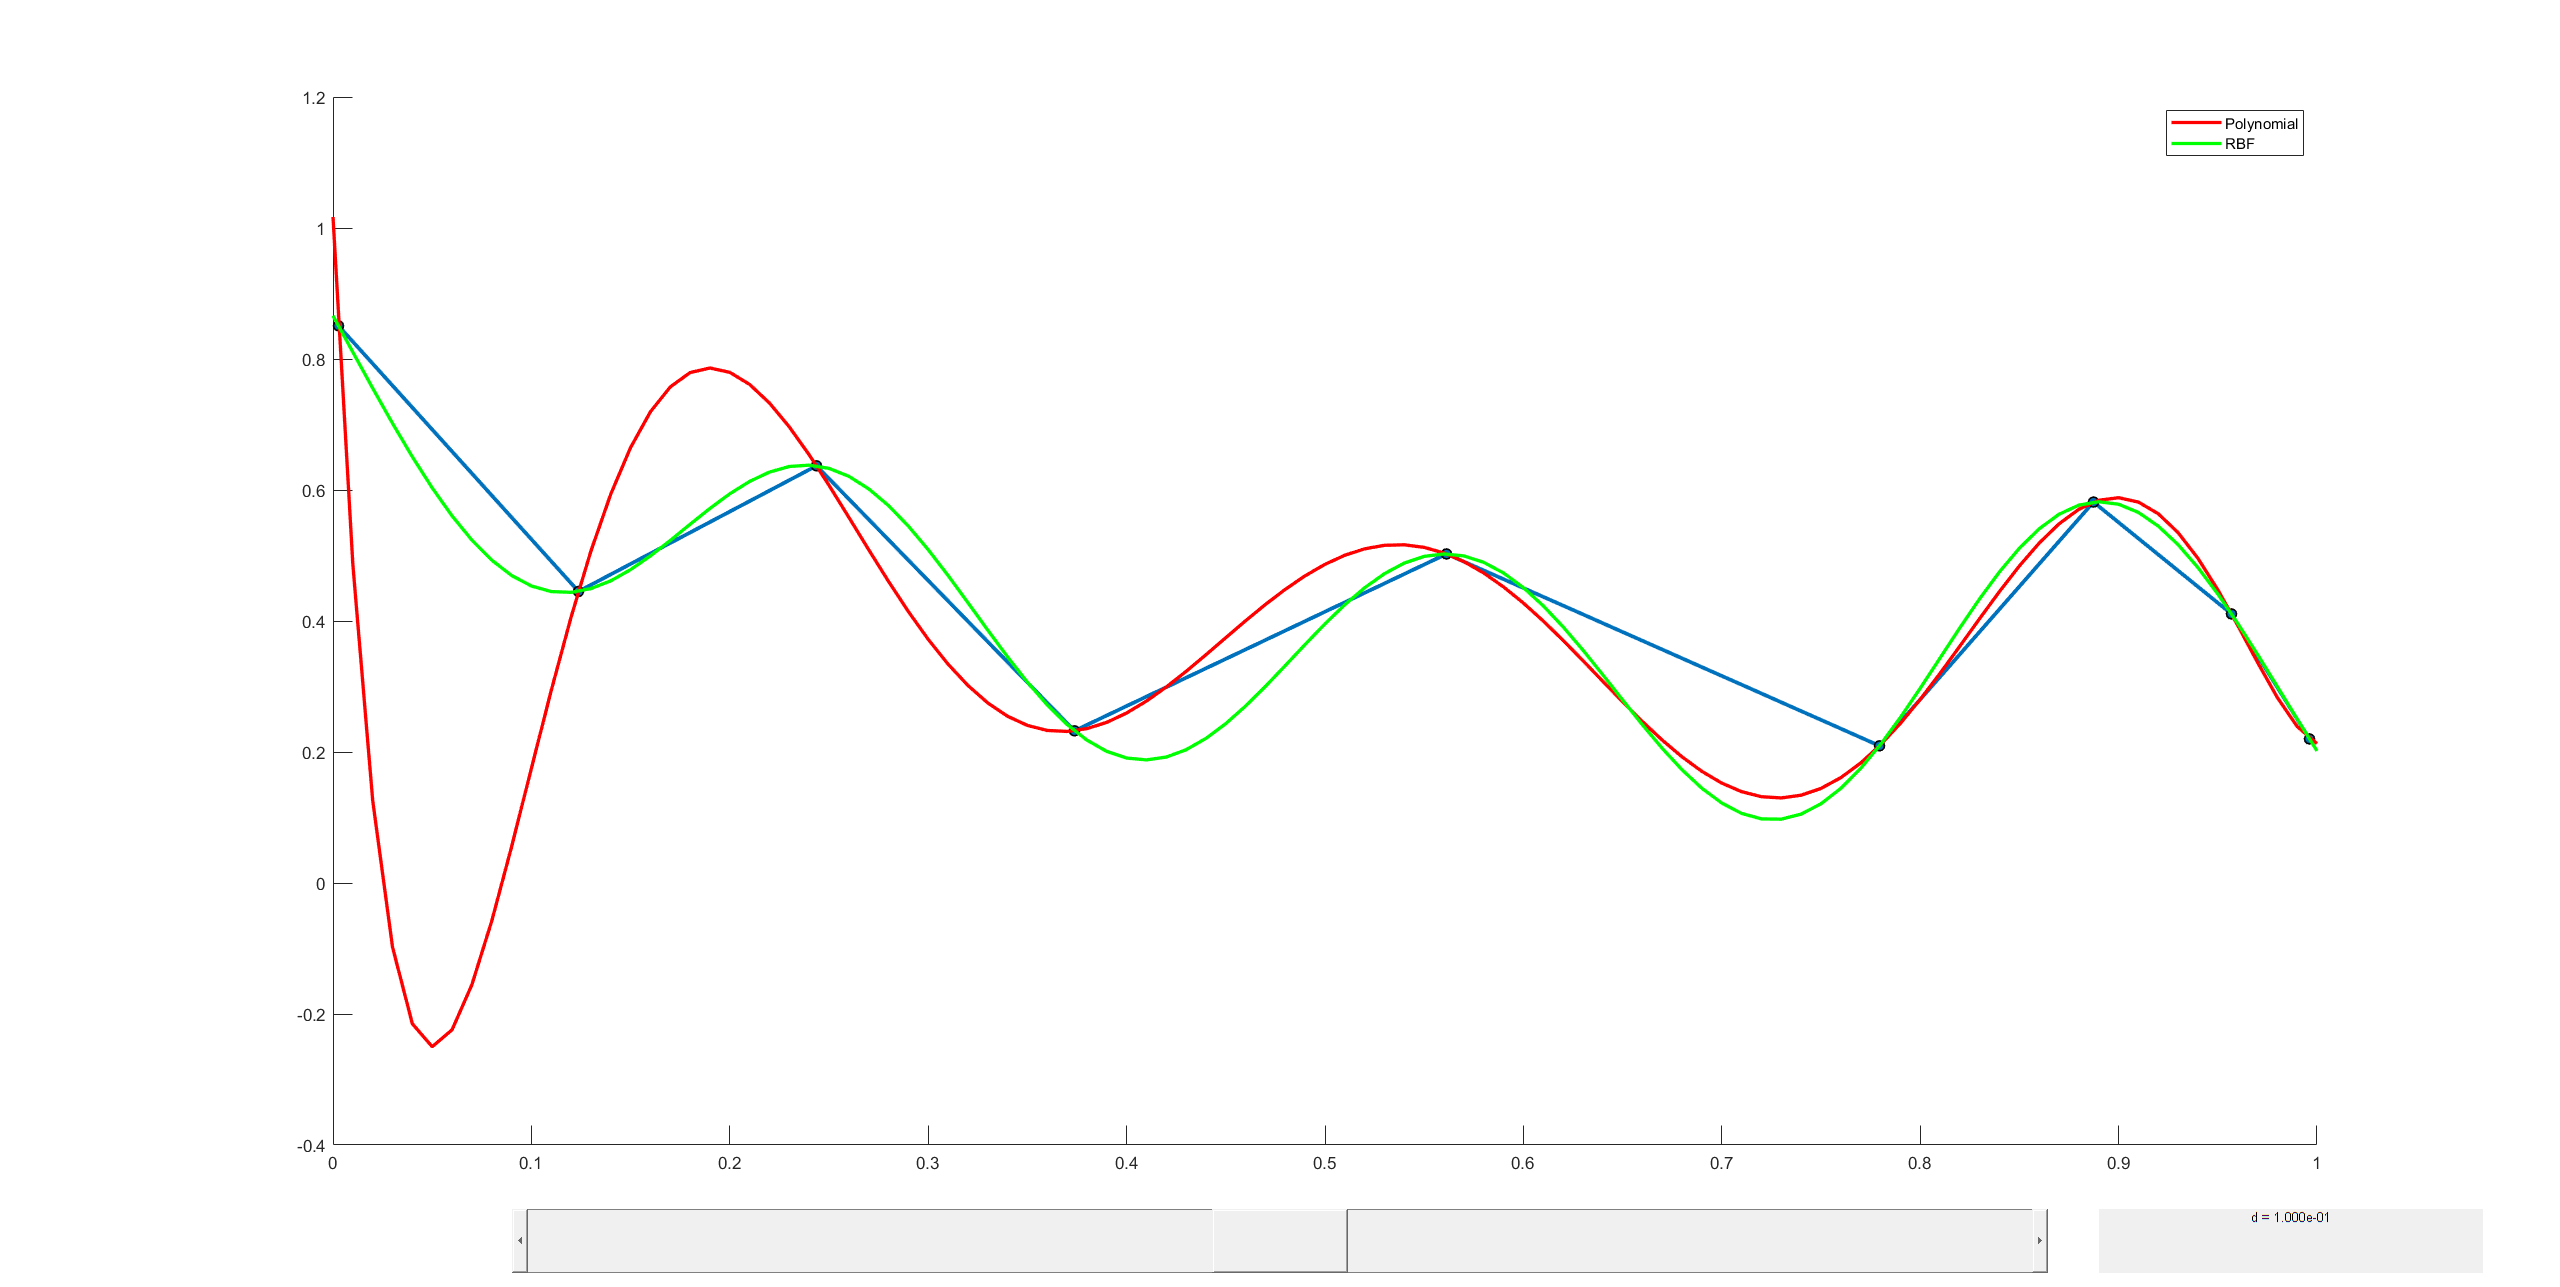
\includegraphics[width=0.45\textwidth]{Figure/20runge.png}%
                \label{fig:runge}%
            }\hfill
            \subfloat[RBF with large d, unstable]{%
                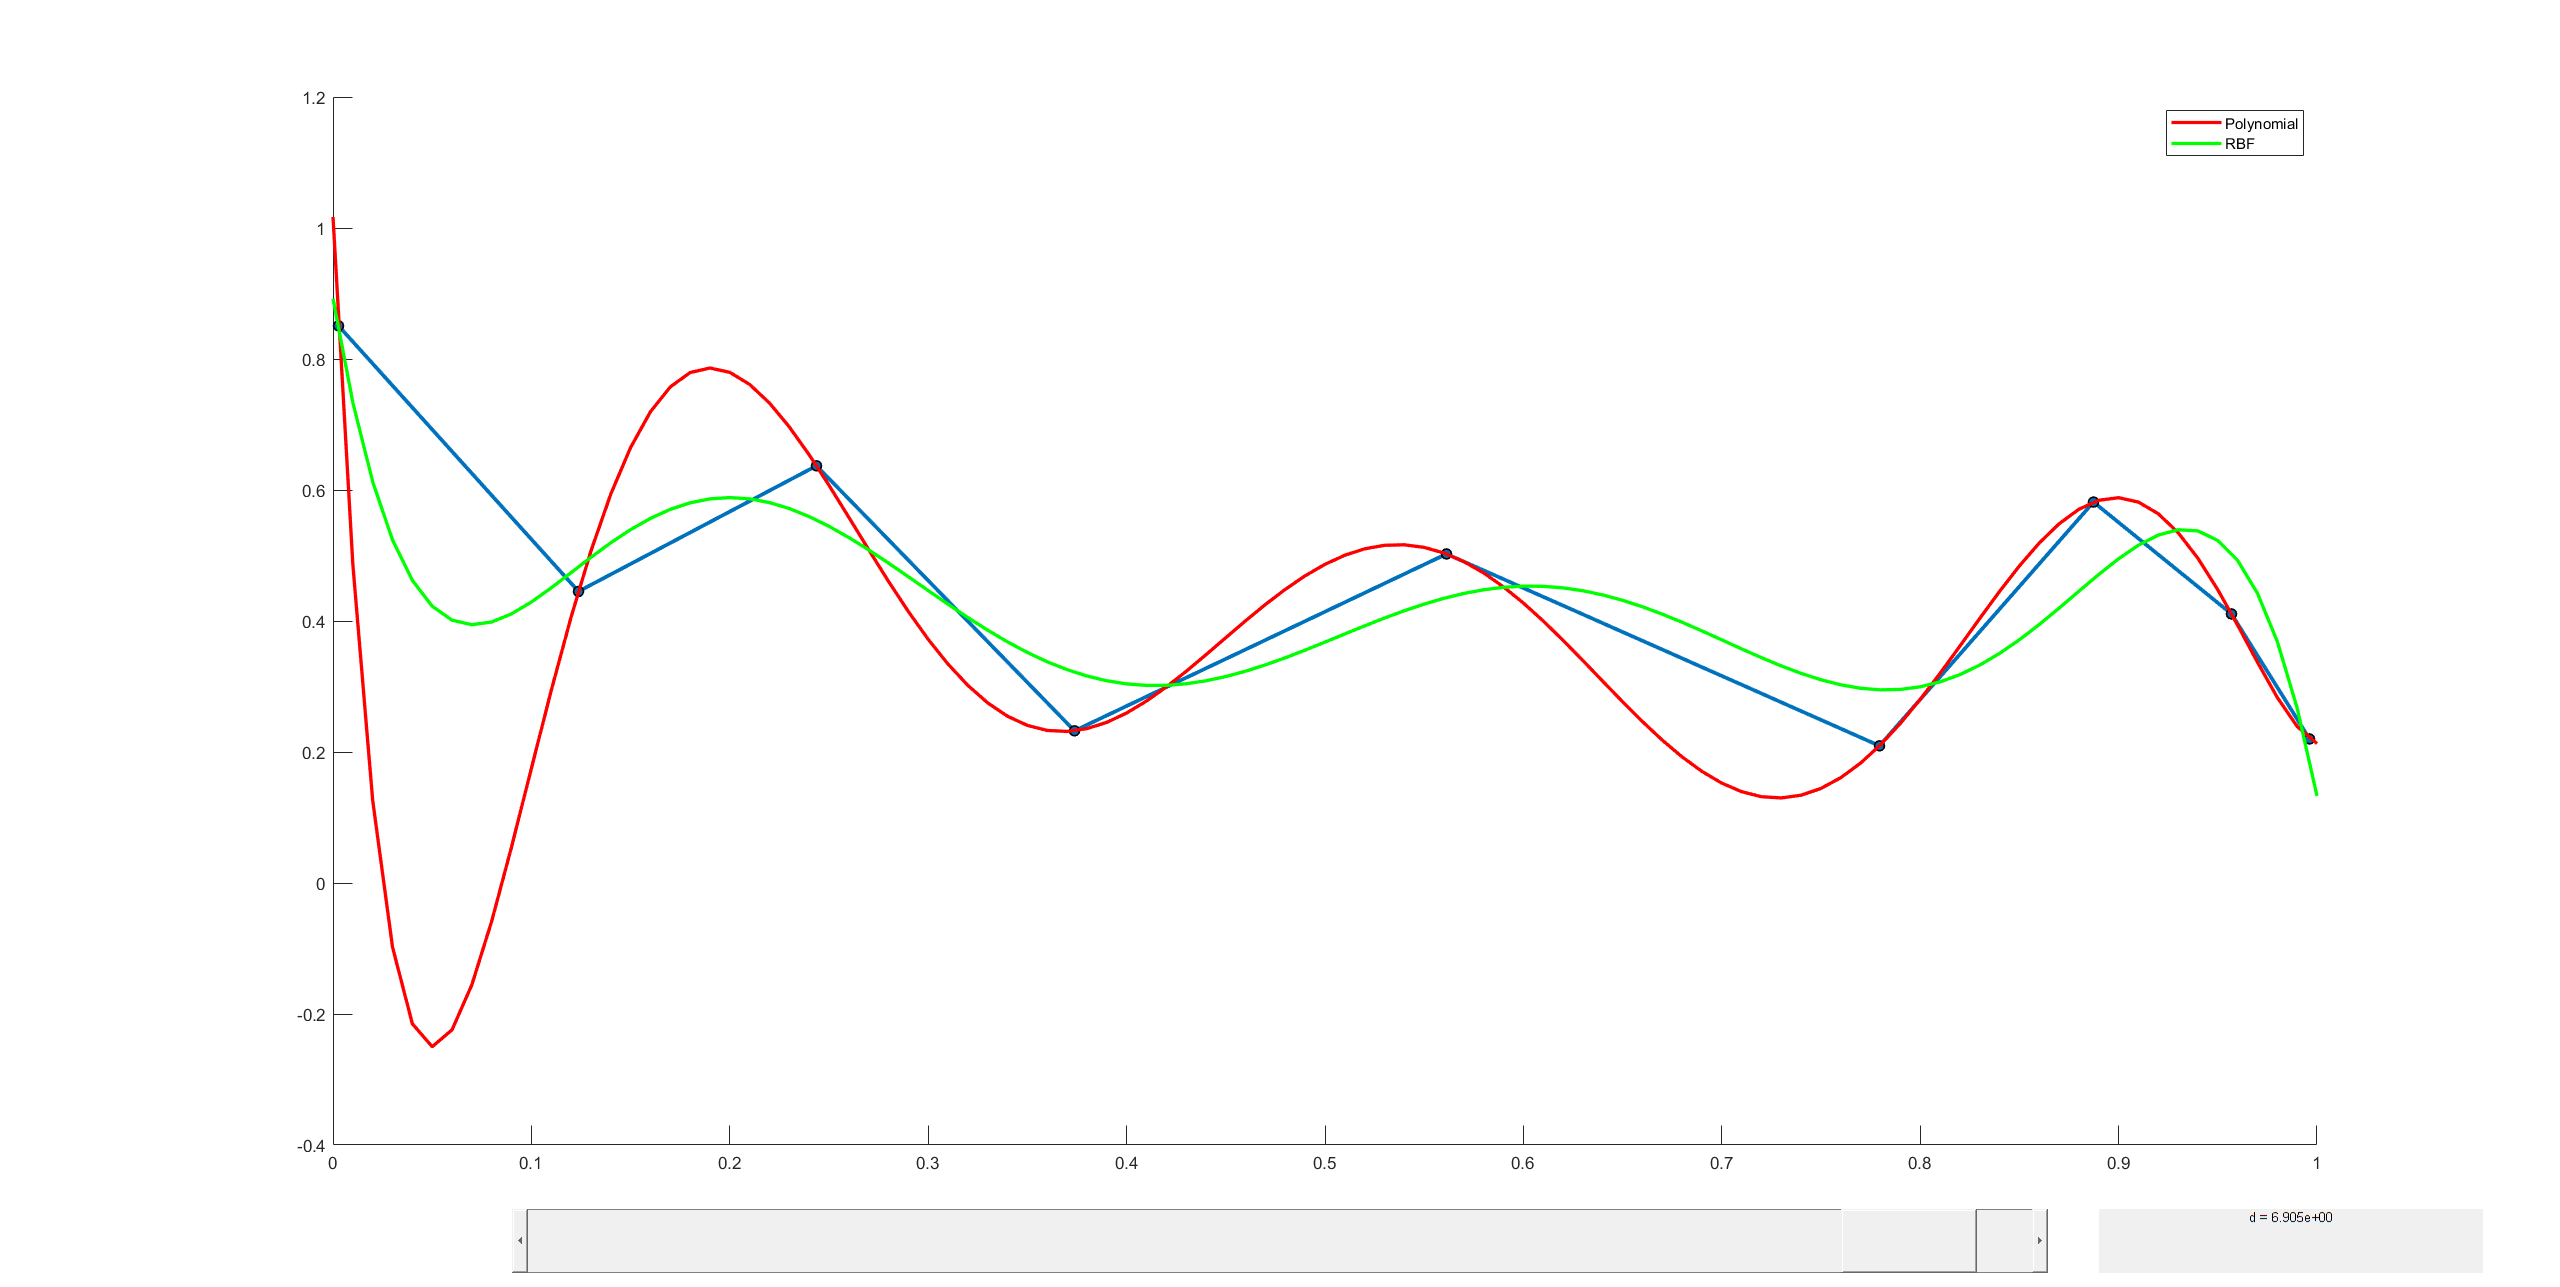
\includegraphics[width=0.45\textwidth]{Figure/21runge_big_d.png}%
                \label{fig:runge_big_d}%
            }

            \caption{Comparison of interpolation methods under different point sets.}
            \label{fig:interpolation_comparison}
        \end{figure}

        \section{Extreme Data Cases}
            Under certain extreme data conditions, such as points with identical x-coordinates, polynomial interpolation may fail to produce results (due to division by zero), and RBF interpolation may not pass through all the given points, as shown in Figure~\ref{fig:extreme}. However, the program does not produce errors or crash.

        \begin{figure}[htbp]
            \centering
            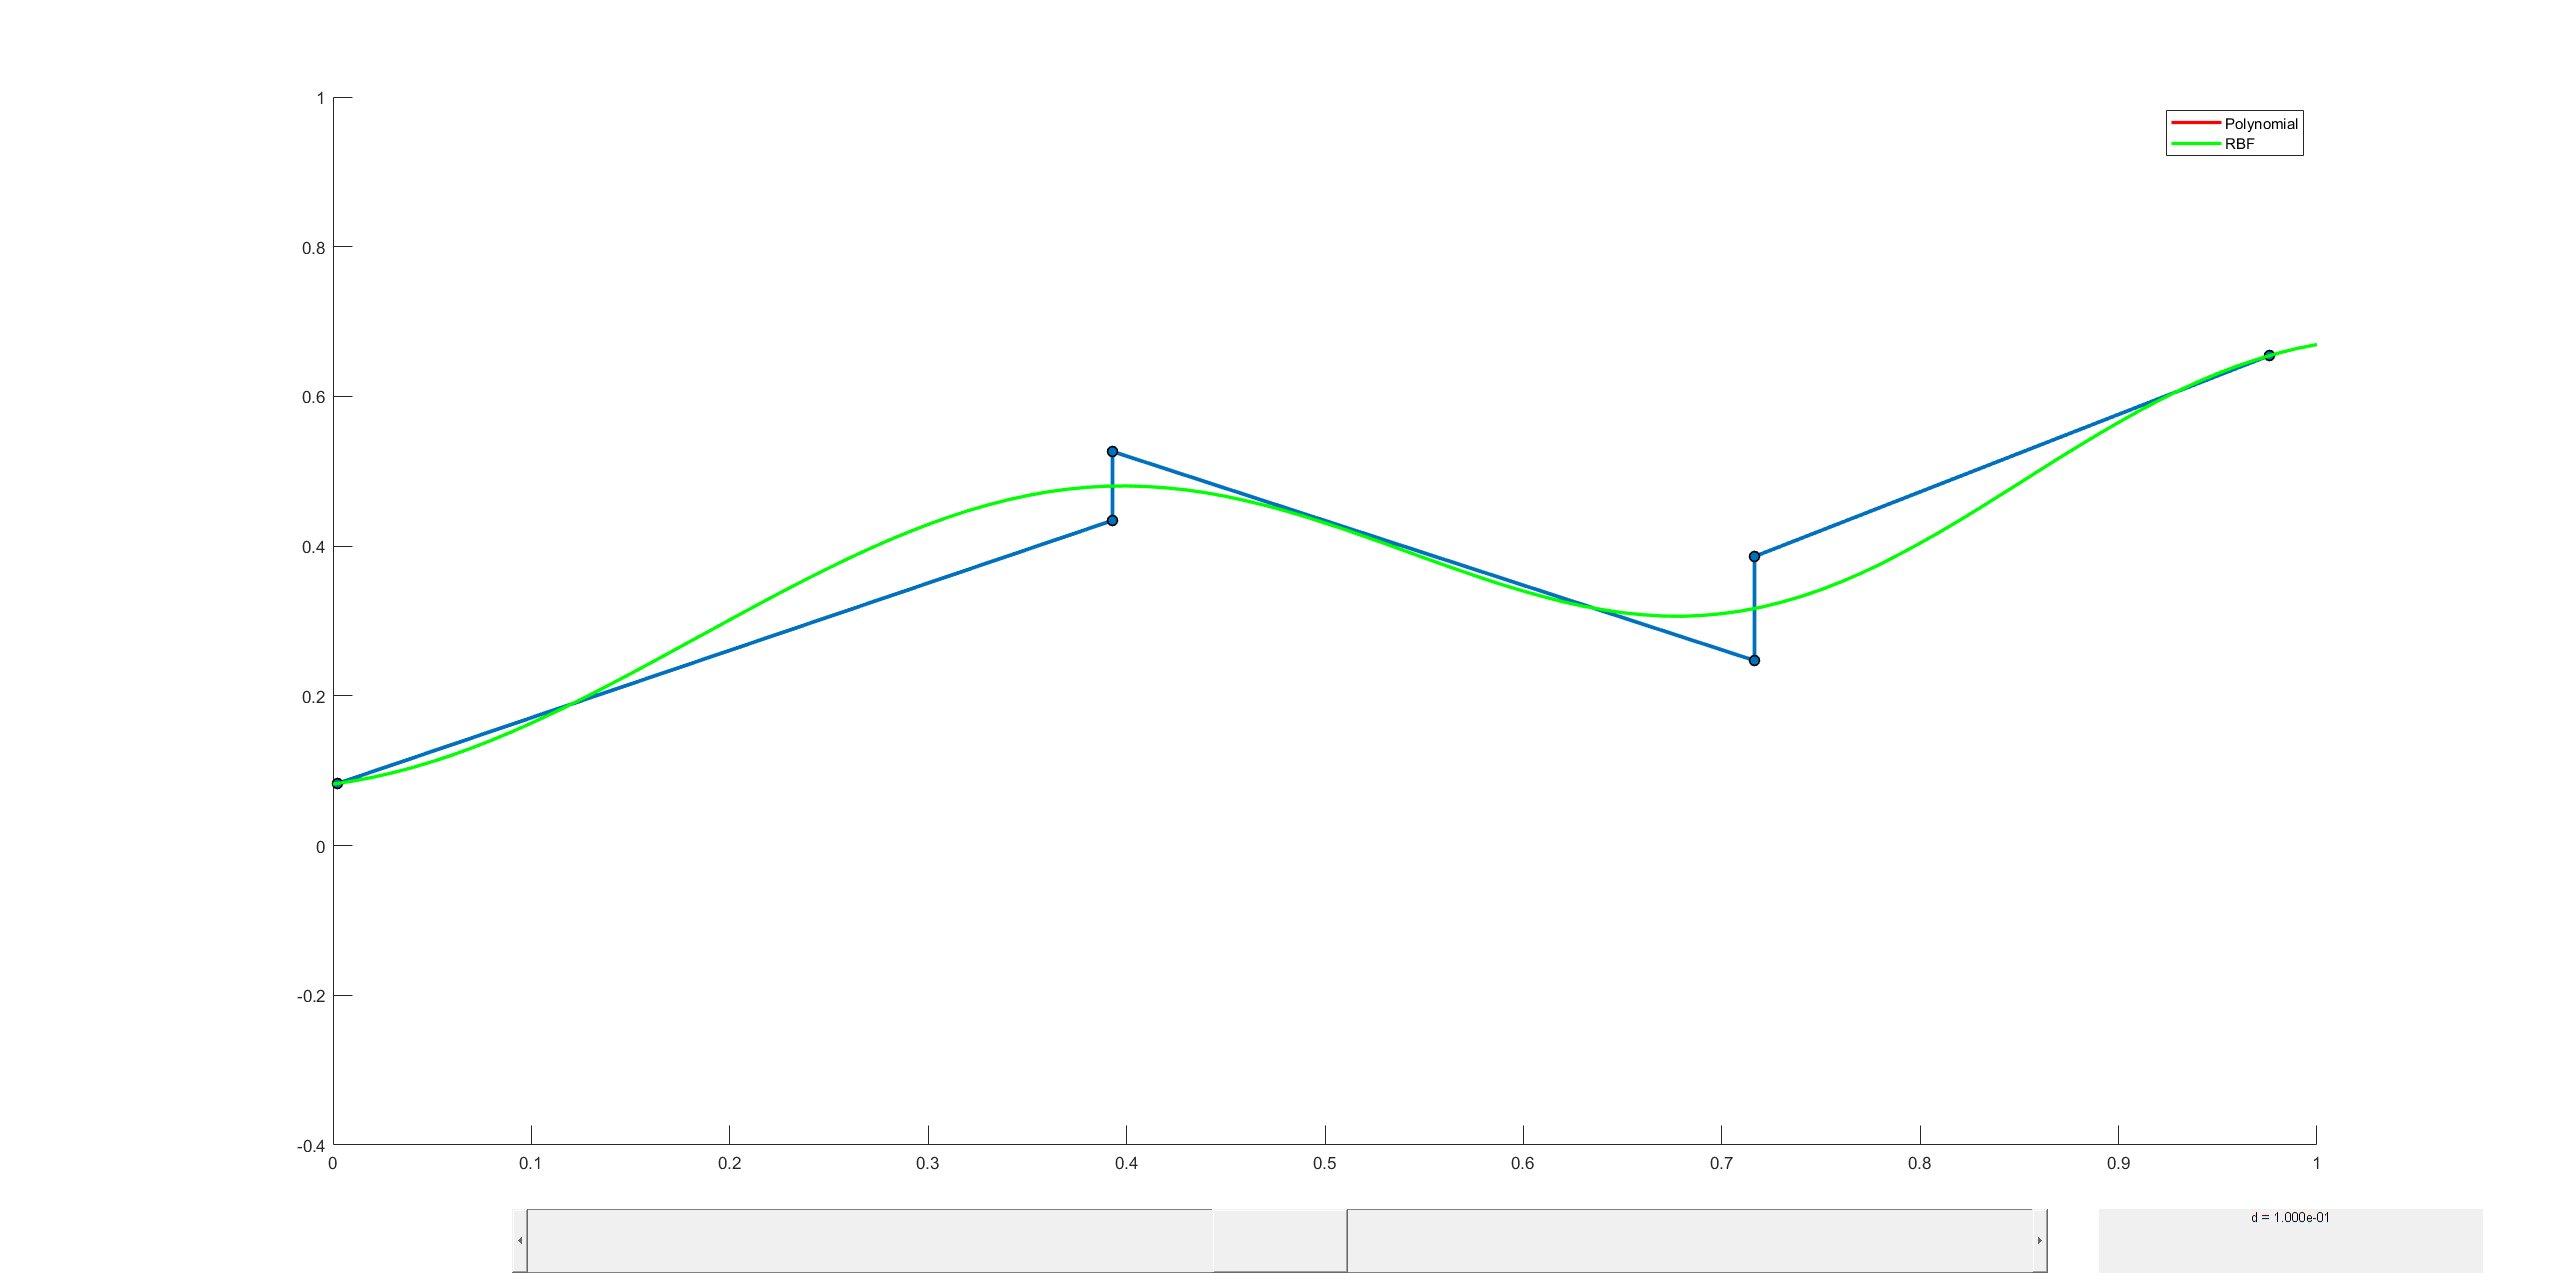
\includegraphics[width=0.6\textwidth]{Figure/30extreme.png}
            \caption{Extreme data cases where polynomial interpolation fails and RBF does not pass through all points.}
            \label{fig:extreme}
        \end{figure}

    \chapter{Discussion}
        In this experiment, we compared the applicability and performance of polynomial interpolation and radial basis function (RBF) interpolation by analyzing different types of point sets. The results indicate:

        \begin{enumerate}
            \item \textbf{Nearly linear points}: Both methods can fit well, but polynomial interpolation may exhibit slight oscillations at the boundaries, especially when the number of points is odd or the spacing between points is uneven. RBF interpolation produces smoother results overall.
            \item \textbf{Convex points}: Polynomial interpolation naturally preserves convexity, whereas RBF interpolation may slightly violate convexity when the shape parameter is small. Increasing the parameter $d$ can improve convexity.
            \item \textbf{Oscillatory points}: Polynomial interpolation is prone to the Runge phenomenon, particularly with a larger number of unevenly spaced points. RBF interpolation is smoother, but overly large shape parameters may compromise numerical stability and prevent the interpolated function from passing through all points.
            \item \textbf{Extreme data conditions}: For points with identical x-coordinates, polynomial interpolation fails due to division by zero, and RBF interpolation cannot pass through all points. However, the program remains stable and does not produce errors or crash.
        \end{enumerate}

        Overall, polynomial interpolation is suitable for a small number of evenly distributed points, while RBF interpolation is better suited for non-uniform or complex point distributions, with adjustable parameters to achieve smooth and stable results.

    \chapter{Questions and Analysis}
        As described in Section~\ref{sec:rbf}, for a constant tail term, only one additional unknown is introduced, so we can add the constraint $\sum_{i=0}^{n-1} b_{i} = 0$ to make the system a symmetric linear system. For higher-order tail terms, similar constraints can be added:
        \begin{equation*}            
            \sum_{j=0}^{n-1} b_{j}\,p_{k}(x_{j}) = 0, \quad k = 0, \dots, m
        \end{equation*}

        This leads to a linear system with a block matrix form:
        \begin{equation*}
            \begin{bmatrix}
                A & P \\
                P^{\top} & 0
            \end{bmatrix}
            \begin{bmatrix}
                \mathbf b \\
                \mathbf c
            \end{bmatrix}
            =
            \begin{bmatrix}
                \mathbf y \\
                \mathbf 0
            \end{bmatrix}
        \end{equation*}
        which can then be solved accordingly.


    \chapter{Conclusion}
        This experiment implemented an interactive visualization tool for both polynomial and RBF interpolation, and the comparison of different point sets leads to the following conclusions:

        \begin{enumerate}
            \item Polynomial interpolation performs well for nearly linear or convex point sets but may exhibit oscillations or numerical issues with oscillatory or extreme data.
            \item RBF interpolation is generally smooth and can handle complex or non-uniform point sets, but proper selection of the shape parameter is required to ensure numerical stability.
            \item The interactive tool allows users to add and move points in real time and adjust RBF parameters, facilitating observation of the strengths, weaknesses, and parameter sensitivity of both methods.
        \end{enumerate}

        The experimental results provide an intuitive reference for understanding the applicability of different interpolation methods and offer a basis for visualizing and analyzing more complex data fitting in future studies.
\end{document}
